\documentclass{beamer}
\mode<presentation>
\usepackage{amsmath}
\usepackage{amssymb}
%\usepackage{advdate}
\usepackage{adjustbox}
\usepackage{subcaption}
\usepackage{enumitem}
\usepackage{multicol}
\usepackage{mathtools}
\usepackage{listings}
\usepackage{url}
\def\UrlBreaks{\do\/\do-}
\usetheme{Boadilla}
\usecolortheme{lily}
\setbeamertemplate{footline}
{
  \leavevmode%
  \hbox{%
  \begin{beamercolorbox}[wd=\paperwidth,ht=2.25ex,dp=1ex,right]{author in head/foot}%
    \insertframenumber{} / \inserttotalframenumber\hspace*{2ex} 
  \end{beamercolorbox}}%
  \vskip0pt%
}
\setbeamertemplate{navigation symbols}{}

\providecommand{\nCr}[2]{\,^{#1}C_{#2}} % nCr
\providecommand{\nPr}[2]{\,^{#1}P_{#2}} % nPr
\providecommand{\mbf}{\mathbf}
\providecommand{\pr}[1]{\ensuremath{\Pr\left(#1\right)}}
\providecommand{\qfunc}[1]{\ensuremath{Q\left(#1\right)}}
\providecommand{\sbrak}[1]{\ensuremath{{}\left[#1\right]}}
\providecommand{\lsbrak}[1]{\ensuremath{{}\left[#1\right.}}
\providecommand{\rsbrak}[1]{\ensuremath{{}\left.#1\right]}}
\providecommand{\brak}[1]{\ensuremath{\left(#1\right)}}
\providecommand{\lbrak}[1]{\ensuremath{\left(#1\right.}}
\providecommand{\rbrak}[1]{\ensuremath{\left.#1\right)}}
\providecommand{\cbrak}[1]{\ensuremath{\left\{#1\right\}}}
\providecommand{\lcbrak}[1]{\ensuremath{\left\{#1\right.}}
\providecommand{\rcbrak}[1]{\ensuremath{\left.#1\right\}}}
\theoremstyle{remark}
\newtheorem{rem}{Remark}
\newcommand{\sgn}{\mathop{\mathrm{sgn}}}
\providecommand{\abs}[1]{\left\vert#1\right\vert}
\providecommand{\res}[1]{\Res\displaylimits_{#1}} 
\providecommand{\norm}[1]{\lVert#1\rVert}
\providecommand{\mtx}[1]{\mathbf{#1}}
\providecommand{\mean}[1]{E\left[ #1 \right]}
\providecommand{\fourier}{\overset{\mathcal{F}}{ \rightleftharpoons}}
%\providecommand{\hilbert}{\overset{\mathcal{H}}{ \rightleftharpoons}}
\providecommand{\system}{\overset{\mathcal{H}}{ \longleftrightarrow}}
	%\newcommand{\solution}[2]{\textbf{Solution:}{#1}}
%\newcommand{\solution}{\noindent \textbf{Solution: }}
\providecommand{\dec}[2]{\ensuremath{\overset{#1}{\underset{#2}{\gtrless}}}}
\newcommand{\myvec}[1]{\ensuremath{\begin{pmatrix}#1\end{pmatrix}}}
\let\vec\mathbf

\lstset{
%language=C,
frame=single, 
breaklines=true,
columns=fullflexible
}

\numberwithin{equation}{section}

\title{Question-Circle}
\author{Mohit \\ EE24BTECH11041}

\date{NOVEMBER 6,2024} 
\begin{document}

\begin{frame}
\titlepage
\end{frame}

\section*{Outline}
\begin{frame}
\tableofcontents
\end{frame}
\section{Problem}
\begin{frame}
\frametitle{Problem Statement}
%
Equation of the circle with centre on the Y axis and passing through the origin and the point $\brak{2, 3}$ is

a) $x^2 + y^2 + 6x + 6y + 3 = 0$\\
b) $x^2 + y^2 - 6x - 6y - 9 = 0$\\
c) $x^2 + y^2 - 6x - 6y + 9 = 0$\\
d) none of these



\end{frame}

\section{Solution}
\subsection{Solution}
\begin{frame}
\frametitle{Solution}

\begin{center}
\begin{table}
  \begin{tabular}[12pt]{ |c| c|}
    \hline
    \textbf{Variable} & \textbf{Description} \\ 
    \hline
    $\vec{x_1}$ & Point on circle \\
    \hline
    $\vec{x_2}$ & Point on circle \\
    \hline 
    $\vec{n}$ &  Normal vector of line at which centre of circle lies \\
    \hline
    $\vec{u}$ & Minus times the coordinate of centre\\
    \hline
    r & Radius of the circle\\
    \hline
    c & Constant in equation of line\\
    \hline
    f & $\norm{\vec{u}}^2$ - $r^2$ \\ 
    \hline   
    \end{tabular}
\end{table}
\end{center}

\begin{align}
	\vec{x}_{1} = \myvec{2\\3},\ \vec{x}_{2} = \myvec{0\\0},\
	\vec{n} = \myvec{1 \\ 0},\  c= 0.
\end{align}
%
The centre is given by
%
\begin{align}
\myvec{
 2 \vec{x}_1 & 2 \vec{x}_2 & \vec{n}
 \\
 1 & 1 & 0
 }^\top 
	\myvec{\vec{u} \\ f} =
-\myvec{ 	\norm{\vec{x}_1}^2 
\\ \norm{\vec{x}_2}^2 	\\c  }
\end{align}
\end{frame}

\subsection{Matrix Equation}
\begin{frame}
\frametitle{Matrix Equation}
Substituting values of $\vec{x}_1$,$\vec{x}_2$ and $\vec{n}$
%\begin{enumerate}[label=(\roman*)]
\begin{align}
	\myvec{
	        4 & 6 & 1\\
	        0 & 0 & 1\\
-1 & 0 & 0}
	\myvec{\vec{u}\\f} = 
	\myvec{-13 \\ 0 \\ 0}
\end{align}
The augmented matrix is expressed as
\begin{align}
	\myvec{
	        4 & 6 & 1 & \vrule & -13\\
	       0 & 0 & 1 & \vrule & 0\\
-1 & 0 & 0 & \vrule & 0}
\end{align}


\end{frame}
\subsection{Row Reduction}
\begin{frame}
\frametitle{Row Reduction}
Performing a sequence of row operations to transform into an Echelon \\form
\begin{align*}
	\xleftrightarrow[]{{R_1\leftrightarrow R_3}}
	\myvec{1 & 0 & 0 & \vrule & 0\\
	        0 &  0 & 1 & \vrule & 0\\
	        4 & 6 & 1 & \vrule & -13}
	\xleftrightarrow[]{{R_3\rightarrow R_3-4R_1}}
	\myvec{1 & 0 & 0 & \vrule & 0\\
	        0 &  0 & 1 & \vrule & 0\\
	        0 &  6 & 1 & \vrule & -13}\\
	\xleftrightarrow[]{{}}
	\myvec{ 1 & 0 & 0 & \vrule & 0\\
	        0 &  1 & \frac{1}{6} & \vrule & -\frac{13}{6}\\
	        0 &  0 & 1 & \vrule & 0}	
	\xleftrightarrow[]{{R_2\rightarrow R_2-\frac{1}{6}R_3}}
	\myvec{ 1 &  0 & 0 & \vrule & 0\\
	        0 &  1 & 0 & \vrule & -\frac{13}{6}\\
	        0 &  0 & 1 & \vrule & 0}
\end{align*}
%
%The radius  of $C$ is obtained as
%\begin{align}
%r = \norm{O-P} = 2
%\end{align}
\end{frame}
%\section{Plot}
\subsection{Results}
\begin{frame}[fragile]
\frametitle{Results}

Thus,the values of $\vec{u}$ and $f$ are
\begin{align}
	\vec{u} = -\myvec{0\\\frac{13}{6}},\
	f = 0.
\end{align}
The radius of circle is
\begin{align}
	r=\sqrt{(\norm{\vec{u}}^2-f)}=\frac{13}{6}
\end{align}
The equation of circle is
\begin{align}
	\norm{\vec{x}}^2-2\myvec{0 & \frac{13}{6}}\vec{x}=0
\end{align}
OR
\begin{align}
x^2+y^2-\frac{13}{3}y=0
\end{align}
Hence,option (d) is correct

\end{frame}
%plots Fig. \ref{fig:circle_diameter}.
%
\subsection{Figure}
\begin{frame}
\frametitle{Figure}
\begin{figure}
\centering
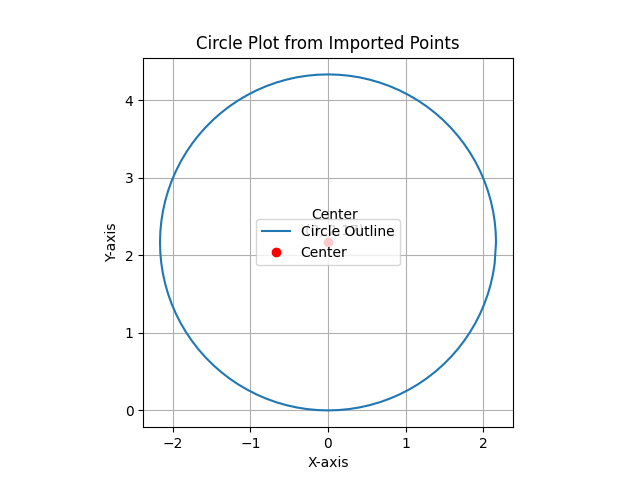
\includegraphics[width=0.6\columnwidth]{figs/Figure_1.png}
\caption{Circle}
\label{fig:circle_diameter}
\end{figure}
\end{frame}

\subsection{C-Code}
\begin{frame}
\frametitle{C-Code}
\lstinputlisting[language=C]{codes/line_gen.c}

\end{frame}
\begin{frame}
\frametitle{C-Code}
\lstinputlisting[language=C]{codes/line_gen2.c}

\end{frame}
\begin{frame}
\frametitle{C-Code}
\lstinputlisting[language=C]{codes/line_gen3.c}

\end{frame}

\subsection{Python-Code}
\begin{frame}
\frametitle{Python-Code}
\lstinputlisting{codes/Question3.py}
\end{frame}
\subsection{Python-Code}
\begin{frame}
\frametitle{Python-Code}
\lstinputlisting{codes/Question32.py}
\end{frame}


\begin{frame}
\frametitle{Python-Code}
\lstinputlisting{codes/Question33.py}
\end{frame}
\end{document}
